\documentclass[a4paper,12pt,twoside,openany]{memoir}
\setheadfoot{28pt}{1cm}

%%% DIVERSE PAKKER %%%
\usepackage{float}

% Listings til kode

\usepackage{listings}
\lstloadlanguages{[Sharp]C}
\renewcommand\lstlistingname{Code example}

\lstset{ %
language=[Sharp]C,              % the language of the code
%basicstyle=\footnotesize,      % the size of the fonts that are used for the code
numbers=left,                   % where to put the line-numbers
%numberstyle=\footnotesize,     % the size of the fonts that are used for the line-numbers
stepnumber=1,                   % the step between two line-numbers. If it's 1, each line 
                                % will be numbered
numbersep=5pt,                  % how far the line-numbers are from the code
%backgroundcolor=\color{white}, % choose the background color. You must add \usepackage{color}
showspaces=false,               % show spaces adding particular underscores
showstringspaces=false,         % underline spaces within strings
showtabs=false,                 % show tabs within strings adding particular underscores
frame=single,                   % adds a frame around the code
tabsize=2,                      % sets default tabsize to 2 spaces
captionpos=t,                   % sets the caption-position to top
breaklines=true,                % sets automatic line breaking
breakatwhitespace=false,         % sets if automatic breaks should only happen at whitespace
%title=\lstname,                % show the filename of files included with \lstinputlisting;
                                % also try caption instead of title
%escapeinside={\%*}{*)},        % if you want to add a comment within your code
%morekeywords={*,...}           % if you want to add more keywords to the set
}

% Dansk orddeling
\usepackage[english]{babel}

%Floats og [H]
\usepackage{float}

% Nummering af eksempler og sætninger
\usepackage{amsthm}
\theoremstyle{definition}
\newtheorem{example}{Example}
\newtheorem{theorem}{Theorem}

% Giver mulighed for at bruge æ, ø og å i .tex-filer
\usepackage[utf8x]{inputenc}

% Hjælper med orddeling ved æ, ø og å. Sætter fontene til at
% være ps-fonte, i stedet for bmp
\usepackage[T1]{fontenc}

% Pakke, der gør det muligt at anvende grafikfiler, samt andvende flere captions på samme figure
\usepackage{graphicx}
\usepackage{caption}
\usepackage{subcaption}

% Pakker, der kan udelades, hvis man ikke gør megen brug af matematik
\usepackage{amsmath}
\usepackage{amssymb}

% Pakke, der kan indsætte nødvendige mellemrum efter
% makro-anvendelser.
\usepackage{xspace}

% Retter forskellige bugs i LaTeX-kernen
\usepackage{fixltx2e}

% Indsæt rettelser og lignende med \fixme{...} med "final"
% i stedet for "draft" udløses en error for hver fixme,
% når der compiles.
\usepackage[footnote,draft,english,silent,nomargin]{fixme}

% Gør det muligt at definere farver.
% Se en.wikibooks.org/wiki/LaTeX/Colors for mere info.
\usepackage{color}
\usepackage[usenames,dvipsnames]{xcolor}

%Hyperlinks i indholdsfortegnelse
\usepackage{hyperref}

%Itemization i tables og andet leg
\usepackage{tabularx}
\usepackage{booktabs} % http://ctan.org/pkg/booktabs
\newcommand{\tabitem}{~~\llap{\textbullet}~~}

\hypersetup{
	bookmarks=true,  % Vis 'bookmark'-ramme.
	colorlinks=true, % True = links har farver, False = links har rammer
	citecolor=black,  % Linkfarve for referencer.
	linkcolor=black,  % Linkfarve i indholdsfortegnelse
	urlcolor=black,   % Linkfarve for eksterne URL'er.
}

%%% LITTERATURLISTE %%%
\usepackage[square,numbers]{natbib}
\usepackage{url}

%%% MARGINER %%%
\setlrmarginsandblock{3.5cm}{2.5cm}{*}	% \setlrmarginsandblock{Indbinding}{Kant}{Ratio}
\setulmarginsandblock{2.5cm}{3.0cm}{*}	% \setulmarginsandblock{Top}{Bund}{Ratio}
\checkandfixthelayout 			% Laver forskellige beregninger og sætter de almindelige længder op til brug ikke memoir pakker


%%% OTHER STUFF %%%
\newcommand{\pdf}{PDF}

\newcommand{\Z}{\ensuremath{\mathbb{Z}}\xspace}

% Kommando, der sikrer ensartede referencer til figurer

\newcommand{\figref}[1]{Figure \ref{#1}}

\newcommand{\mgd}[2]{\ensuremath{\{ #1 \mid #2 \}}}

%\newtheorem{saetning}{S�tning}
\newtheorem{definition}{Definition}




\usepackage{cleveref}
\crefname{listing}{code example}{code examples}
\usepackage{todonotes}

% Valg a kapiteludseende
\definecolor{numbercolor}{gray}{0.7}			% Definerer en farve til brug til kapiteludseende
\newif\ifchapternonum

\makechapterstyle{jenor}{									% Definerer kapiteludseende -->
  \renewcommand\printchaptername{}
  \renewcommand\printchapternum{}
  \renewcommand\printchapternonum{\chapternonumtrue}
  \renewcommand\chaptitlefont{\fontfamily{pbk}\fontseries{db}\fontshape{n}\fontsize{25}{35}\selectfont\raggedleft}
  \renewcommand\chapnumfont{\fontfamily{pbk}\fontseries{m}\fontshape{n}\fontsize{1in}{0in}\selectfont\color{numbercolor}}
  \renewcommand\printchaptertitle[1]{%
    \noindent
    \ifchapternonum
    \begin{tabularx}{\textwidth}{X}
    {\let\\\newline\chaptitlefont ##1\par} 
    \end{tabularx}
    \par\vskip-2.5mm\hrule
    \else
    \begin{tabularx}{\textwidth}{Xl}
    {\parbox[b]{\linewidth}{\chaptitlefont ##1}} & \raisebox{-15pt}{\chapnumfont \thechapter}
    \end{tabularx}
    \par\vskip2mm\hrule
    \fi
  }
}																						% <--

%\chapterstyle{jenor}
\usepackage{calc,color}
\newif\ifNoChapNumber
\newcommand\Vlines{%
\def\VL{\rule[-2cm]{1pt}{5cm}\hspace{1mm}\relax}
\VL\VL\VL\VL\VL\VL\VL}
\makeatletter
\setlength\midchapskip{0pt}
\makechapterstyle{VZ43}{
\renewcommand\chapternamenum{}
\renewcommand\printchaptername{}
\renewcommand\printchapternum{}
\renewcommand\chapnumfont{\Huge\bfseries\centering}
\renewcommand\chaptitlefont{\Huge\bfseries\raggedright}
\renewcommand\printchaptertitle[1]{%
\Vlines\hspace*{-2em}%
\begin{tabular}{@{}p{1cm} p{\textwidth-3cm}}%
\ifNoChapNumber\relax\else%
\colorbox{black}{\color{white}%
\makebox[.8cm]{\chapnumfont\strut \thechapter}}
\fi
& \chaptitlefont ##1
\end{tabular}
\NoChapNumberfalse
}
\renewcommand\printchapternonum{\NoChapNumbertrue}
}
\makeatother
\chapterstyle{VZ43}



\setsecnumdepth{subsection}		 					% Dybden af nummerede overkrifter (part/chapter/section/subsection)
\maxsecnumdepth{subsection}							% Ændring af dokumentklassens grænse for nummereringsdybde
\settocdepth{subsection} 							% Dybden af indholdsfortegnelsen


%%% FORSIDE %%%
%\title{Dette er rapportens titel}
%\author{Forfatter 1 \\ Forfatter 2}
%\date{November 2011}

% Sørger for LaTeX ikke strækker teksten ved at forhindre
% der bliver tilføjet linieskift, hvis siden ikke er
% fyldt helt ud.
\raggedbottom 



\begin{document}

%%  A simple AAU report template.
%  2012-04-20 v. 0.2.0
%  Copyright 2010-2012 by Jesper Kjær Nielsen <jkn@es.aau.dk>
%
%  This is free software: you can redistribute it and/or modify
%  it under the terms of the GNU General Public License as published by
%  the Free Software Foundation, either version 3 of the License, or
%  (at your option) any later version.
%
%  This is distributed in the hope that it will be useful,
%  but WITHOUT ANY WARRANTY; without even the implied warranty of
%  MERCHANTABILITY or FITNESS FOR A PARTICULAR PURPOSE.  See the
%  GNU General Public License for more details.
%
%  You can find the GNU General Public License at <http://www.gnu.org/licenses/>.
%
%\pdfbookmark[0]{Front page}{label:frontpage}%
%\begin{titlepage}
	%\addtolength{\hoffset}{0.5\evensidemargin-0.5\oddsidemargin} % set equal margins on the frontpage - remove this line if you want default margins
	\thispagestyle{empty}
%	\ThisTileWallPaper{\paperwidth}{\paperheight}{billeder/aau_cover.png}

	\vspace*{\fill}

	\noindent \colorbox{gray}{
		\parbox{\textwidth}{%
			\color{white}%
			\begin{center}
				\Huge{{\fontfamily{ua1}\selectfont Title}} % insert your title here
			\end{center}
			\begin{center}
			\Large{\textsf{Group sw702e14}}\\
			[0.5cm] % insert your subtitle here
			\small{
			%Names here\\
			}
			\end{center}
		}}
		
	\vfill


	\begin{figure}[htbp]
	\centering
	%\includegraphics[width=90mm]{billeder/...}
	\vspace{140px}
	\end{figure}
	
	\noindent \colorbox{white}{
		\begin{minipage}[b]{6.5cm}
		\begin{center}
		%	\includegraphics[width=150px]{billeder/aau_new_logo}
			\end{center}
			\vspace*{-20px}
			%{\small \textcolor{aaublue}{Department of Computer Science}}  \\
			%{\small \textcolor{aaublue}{Software Engineering}}
		\end{minipage}
	} 
	\hfill  
	\colorbox{white}{ 
		\begin{minipage}[b]{3.5cm}	 
			\flushright
			{\large Fall 2014} \\
		\end{minipage}
	}

%\end{titlepage}
\clearpage

%\cleardoublepage

%\frontmatter
%%\Blankpage
\phantomsection
\thispagestyle{empty}
% Titlepage [START]
    \sectionmark{Titlepage}

    \begin{tabular}{r}
        \parbox{\textwidth}{\raisebox{-15mm}{
\includegraphics[height=3cm]{billeder/aauLogoEnStudent.png}} %
         \hfill \parbox{4.9cm}{ %
            \begin{tabular}{l} 
                {\textsf{\small{\textbf{Department of Computer Science}}}}\\
                {\textsf{\small{\textbf{Software 7th semester}}}}\\
                {\textsf{\small{Address: Selma Lagerlöfs Vej 300}}} \\
                {\textsf{\small{\hspace{14 mm} 9220 Aalborg Øst }}} \\
                {\textsf{\small{Phone no.: 99 40 99 40}}} \\
                {\textsf{\small{Fax no.: 99 40 97 98}}} \\
                {\textsf{\small{Homepage: \url{http://www.cs.aau.dk}}}}
            \end{tabular}}}
    \end{tabular}
    
    \begin{tabular}{cc}
	
        \parbox[3cm]{7cm}{ %
	\vspace{7mm}
            \begin{description}
                \item {\textbf{Project title}:} \\
                    A Multiplayer Game Development Framework
                    \hspace{4cm}
                \item {\textbf{Subject}:} \\
                    Internet Technology
            \end{description}
	\vspace{-4mm}
            \parbox{8cm}{ %
                \begin{description}
                    \item {\textbf{Project periode}:} \\
                        Fall 2014
                    \hspace{4cm}
                    \item {\textbf{Group name}:} \\
                        sw702e14
                    \hspace{4cm}
                    \item {\textbf{Supervisor}:} \\
                        Ivan Aaen
                    \item {\textbf{Group members}:}\\%\newcommand{\sh}{18pt}\\%
                    Casper Holst Laustsen\\[0.20cm]
                    Christoffer Nduru\\[0.20cm]
                    Dan Skøtt Petersen\\[0.20cm]
                    Johan Leth Gregersen\\[0.20cm]
                    Kristian Mikkel Thomsen\\[0.20cm]
                    Morten Møller Jakobsen
                \end{description}
            }
	    \vspace{-4mm}
            \begin{description}
                \item {\textbf{Copies}:} 8
                \item {\textbf{Pages}:} \pageref{LastPage}
                \item {\textbf{Appendices}: 0} 
                \item {\textbf{Finished}: 18/12/2014} 
            \end{description}
            \vfill 
        } &
        \parbox{7cm}{ %
            %\vspace{.15cm} %
            \hfill %
            \begin{tabular}{l}%
                {\textbf{Abstract}:}\bigskip \\%
                \fbox{ %
                    \parbox{6.2cm}{\bigskip %
                    {\vfill{\small %
                     %Purpose: To give readers a quick identification of the basic content of the thesis. It should “stand on its own” and be a self-contained document. There should be no need to look elsewhere in the thesis for an understanding of what is said in the abstract.
%1: Objectives and scope
%2: A description of the methods used
%3: A summary of the results
%4: A statement of the main conclusions
                        \bigskip}}%
                    }}%
            \end{tabular}%
        }
    \end{tabular}

    \noindent{\footnotesize\emph{The material in this report is freely and publicly available, publication with source reference is only allowed with authors' permission.}}
% Titlepage [END]
%\Blankpage

%\cleardoublepage


% De vigtigste forskelle mellem \include og \input ligger i at
% \include kun må findes EFTER preamblen og at 
% inkluderede filer kan fravælges ved generering af output
% ved brug sammen med \includeonly.

% Se arbejdsblad-skabelon.tex for et eksempel herpå.

%\thispagestyle{empty}
\section*{Preface}
This report was written by six 7th semester software engineering students from Aalborg University.\\

\noindent The report documents the development of a framework for meant for developing location-based multiplayer games.

\noindent The source code for this project including raw test data is accessible through one of the following links:
\begin{itemize}
\item \url{http://goo.gl/MjpyXz}
\item \url{https://www.dropbox.com/s/9y1zmsq3evn5vu5/sw702e14_SOURCE.zip}
\end{itemize}

\vspace{.2cm}
\noindent We would like to thank our supervisor Ivan Aaen for providing guidance and feedback.

\begin{table}[H]
	\centering
	\vspace{2cm}
		\begin{tabular}{c c c}
			\underline{\phantom{JAERJAERJAERJAERGO}} & \phantom{cookies} & \underline{\phantom{JAERJAERJAERJAERGO}} \\
			Casper Holst Laustsen & \phantom{cookies} & Christoffer Ndũrũ\\[1.5cm]
		    \underline{\phantom{JAERJAERJAERJAERGO}} & \phantom{cookies} & \underline{\phantom{JAERJAERJAERJAERGO}} \\
			Dan Skøtt Petersen & \phantom{cookies} & Johan Leth Gregersen\\[1.5cm]
			\underline{\phantom{JAERJAERJAERJAERGO}} & \phantom{cookies} & \underline{\phantom{JAERJAERJAERJAERGO}} \\ 
			Kristian Mikkel Thomsen & \phantom{cookies} & Morten Møller Jakobsen\\[.5cm]				
		\end{tabular}
\end{table}


% For at sikre sideskift efter forord. Denne kommando bør kun bruges i
% absolutte undtagelsestilfælde.

%\newpage
\mainmatter
\tableofcontents*
\newpage

%Main parts of report
%\listoffixmes
%INTRODUCTION
%\chapter{Introduction}
\label{chap:intro}
%http://thesistips.wordpress.com/2012/03/25/how-to-write-your-introduction-abstract-and-summary/

% It introduces the problem and motivation for the study.

% - Tell the reader what the topic of the report is.
% - Explain why this topic is important or relevant.

% It provides a brief summary of previous engineering and/or scientific work on the topic.
% - Here you present an overview what is known about the problem.  You would typically cite earlier studies conducted on the same topic and/or at this same site, and in doing so, you should reveal the yawning void in the knowledge that your brilliant research will fill.

% It outlines the purpose and specific objectives of the project.
Development of an online multiplayer game serving many users can be split into two parts: Creating the actual game functionality, and creating the underlying architecture to support it. When developing new games these parts are possibly mixed together as the underlying architecture is only used for the specific game. This has the consequence that the developer possibly writes a game specific architecture, and not a general architecture. In some cases, the developer may want to create other similar games with the same underlying structure, but since the architecture and the game itself are intertwined, it is difficult to reuse the same structure. The developer would have to first search through the previous model and extract the desired features, which costs some time. Furthermore, the functionality might not be an exact match to the needs of the new game, requiring additional time to adjust the code.

The focus of this project is to create a flexible and reliable architecture for a server that supports client based multiplayer games. The goal is to allow easy development of multiplayer games for smartphones, and to make it possible for developers to focus on the game development without having to worry about managing the underlying architecture.

The framework will focus on creating a platform for games centered around the location of the player. It has to be scalable, and therefore the server should easily be able to handle multiple games and multiple devices (players) at the same time. This means it is a requirement that multiple clients should be able to connect to the server and perform different actions at the same time. The framework should be able to handle GPS-coordinates, using it as the base of some sort of action, depending on the game implementation of the game, e.g. in a shooter game you are able to shoot players within a certain distance. 

Creating new games from scratch requires both time and monetary investments. While some companies might have these resources available, it could increase the potential profit if some of these resources could be saved. The extra time either means a bigger profit for the developer or more time to work on game features. We argue that creating a flexible framework could help improve this situation.

A framework serves as a basic set of functionality and structural guidelines for the game to be built upon. Overall, game development rarely fits traditional software development process, such as the waterfall method, as requirements can change quickly, and therefore an agile development process is often used \cite{Gamedevelopment}. This means that functionality might have to change on a frequent basis, and whether this means adding new functionality or rewriting already existing functions, a game with an intertwined framework and game will take more time to rewrite, because components often have or provide dependencies for other parts. Therefore it is important to have a clear seperation of the framework and the game.\\

Consider a third person shooter game where functionality revolves around specific gun types and their properties. Far into the development, another gun type might be a new requirement. The developer would, depending on the existing framework have to rewrite much of the code regarding guns in general to suddenly include new functionality. This requires a lot of extra time compared to having a framework that allows easy addition and removal of gun functionality. It is even worse if you end up having to abandon an idea and create something entirely different. Having to rewrite all the code would be tedious, especially when it involves the framework. Having an independent framework could help alleviate this issue.

The size and the amount of divisions of a developing company also matters. The more different people working on a project, the more precision is needed both in the documentation and the framework. Having multiple people writing code on the same game requires the underlying architecture to be as consistent as possible. Changing something in the framework or the underlying architecture requires a notification to all different divisions and people working on the game and it may result in some code refactoring to accommodate the changes \cite{Gameprod}. According to \citet{Gamedesign}, the big companies often create their own framework and document it through the game design document in order for it to fit exactly their needs. This causes them to have a consistent and steady framework to work on, and work individually without consulting different divisions. Smaller companies may not have the luxury of creating a completely game specific framework for each of their projects resulting in them having to spend more work hours adjusting their code to what their co-developers have coded.

Another problem with developing different games from scratch as opposed to having a standardized framework is compatibility. Having different types of devices with different versions of various operating systems means that some devices might not be compatible with the program. What this means is that programs act differently on different devices. With an existing framework this only has to be implemented once. Having a framework that is already compatible with the different devices allows the developers to focus solely on the game, and therefore limiting the amount of time needed for creating portable code.

Constructing a framework that can be used by different developers could save the developer a lot of time and money if the developer uses the framework as intended. It could and should make it easier for the developer to produce code, giving him less work hours needed to create the same content he otherwise would. The struggle with creating a framework like this is that it has to be flexible enough for game developers to create diverse games, but still be precise enough for the developers to not have to write an a lot of code, in order to fit it to the game.

The goal is widely pursued in the form of game engines and general APIs. A large amount of games being developed, are developed on top of already existing game engines. An example of a game engine is the `Adventure Game Studio', providing an API for creating games in third person perspective along with support for pre-rendering. The developer, Chris Jones, has created different functionality he deemed important for creating these games and published it in the form of a simple IDE for game developers \cite{adv-game}. It is specific in the way it focuses on third person adventure games, includign functionality that is relevant for this type of game.
Another example of game engines, is full blown engines with multiple purposes for a specific genre. One of the most used engines for first person shooters is the "Unreal Engine" which is used for many major shooter or fighter games. It is used both as a visual aid, providing 3D rendering, but also provides pre-rendering functionality.

% It provides a ‘road map’ for the rest of the report.
% - This is so that the reader knows what’s coming and sees the logic of your organization.
% - Describe (in approximately one sentence each) the contents of each of the report/thesis chapters.

\section{Problem Statement}
\label{sec:probstate}
When creating games time and money are valuable resources. To ensure a high amount of quality code, the developer has to spent a lot of time writing code that could be found in a generic framework, increasing the cost unnecessarily. This naturally raises the question:

%\mbox{\parbox[b][2.5cm][c]{0.95\textwidth}{\textit{How can we develop a framework for creating multiplayer games - increasing the experience for the developers.}}}

\mbox{\parbox[b][2.5cm][c]{0.95\textwidth}{\textit{How can a flexible framework for creating multiplayer games be developed?}}}\fxfatal{Bør stadig overvejes!}

\noindent The idea is simple: we want to create a framework for creating simple location-based multiplayer shooter games. In order to properly answer the stated problem, these goals should be fulfilled:

\paragraph{Flexibility} The framework has to be as flexible as possible. I.e., it should allow implementation of as broad a spectrum of games as possible within the mentioned genre.
\paragraph{Scalability} The framework should be able to handle multiple games, each with multiple users. The purpose of hosting several games at once is to allow development of relatively short games with a limited number of players each, e.g. a group of friends.
\paragraph{Ease of Use} The framework has to be easy to use for developers. If it is too complicated it will not be as attractive to start using - the idea is to make development easier rather than harder.





%Scenarios
%\section{Scenario 1: Maps \& Navigation - City Areas}
In a large city, for example one of the 5 largest cities in Denmark, data connectivity can be obscured by many big buildings, concrete parking garages or when entering the the subway. This type of data connection loss can be unpredictable and happen in an instant, but it can be expected to be relatively short. 

A scenario can be a travelling salesman arriving at an unknown large city. The salesman is trying to find a customer and have to navigate through public transportation. The customer is awaiting the salesman for a business meeting, and therefore the salesman is limited by time. The salesman is relying on information about public transport timetables and a journey planner to direct him to the customer. 

A number of challenges may arise for the salesman regarding connectivity issues. The salesman may have plans to ride one bus to the customer, but upon arriving at the bus stop he realises the bus is delayed. He now has to consult his device for an alternative bus to ride. Since the salesman is under time pressure, he is relying heavily on having data-connection. Another challenge may arise if the salesman descents into the metro-station. The salesman may have become confused about which train to enter, and is now relying on still having a data connection. The subway is underground and built from concrete, which may severely reduce the strength of the data connection. 

The challenges arise when the salesman is under time pressure and has to deal with unpredictable traffic and public transportation. The salesman would be more secure if a service would be able to provide the desired information even if the device has lost data-connection.
%\section{Scenario 2: Maps \& Navigation - Countryside Areas}
When travelling out of cities, data connectivity can be unavailable for a longer period of time. This type of data connection loss is slowly fading away as you move further away from the connection source.

A scenario can be a couple going for a walk in the woods on the countryside. They are visiting an unknown area and walks into the woods. They happen to get lost and wants to find their way back to the car, but in the woods no data connection is available and they are lost.

A modification of this scenario could be a couple that wants to get additional knowledge of the area they are walking around in, e.g. visiting Rold skov in Denmark, they might want to read the stories about the robbers from Rold. It is also possible that they want to know about the attractions in the area, and directions to them.

The challenges are predicting that the data connection will be lost in the near future, and what services should be attempted to download to a mobile device. 

%\section{Scenario 3: Bus and Train}
In this scenario the problem be solved is to minimize Internet drop-outs when travelling on frequently used bus or train lines. The idea is to collect data on a user base and use that data to identify areas where the user might lose connection.

The solution should be able to detect travelling by bus or train and predict the route and destination. It should reduce the user experience of no Internet during the travel and make relevant information available for the destination, should it be in a poorly connected area.



%In order to do so several approaches are available.

%A simple approach is to measure the signal strength of the device and use that as the base for predicting when connection will be unavailable. Using this method a stable but slowly dropping signal strength might indicate a future with no connection available, in this event the required web resources should be cached so they are available doing an offline period. Another scenario could when the signal is unstable but the average remains high, this could indicate interference in the area but no risk of a significant offline period, in this case caching is not necessary.
%
%Another approach is to base the prediction on historical data of the near area. This can be done by gathering data of where Internet connections usually drops and build a map for the available providers. Then the caching will be done when a device is predicted to move into such an area.

%Problem statement
% How can a user be guaranteed to always have relevant information available, regardless of network connectivity?
\section{Chapter Descriptions}
The following is a brief description of each chapter in the report

% add more here as report progresses %
\paragraph{From Idea to Framework}
This chapter will give a general idea behind the choices made - why we chose to make a game and what outcome expect to get from it. It will give a short description of the overlying architecture and goal of the framework. 
\paragraph{The Game}
This chapter will describe the game we used a foundation for creating a framework. It will describe the client, how it was designed and lastly how it was implemented.
\paragraph{The Framework}
This chapter describes all of the choices considered for the framework. It will describe how the game influenced the server and framework and advantages and disadvantages of this. Furthermore it will describe design and implementation of the server and database. Lastly a section will describe tests and the result of it.
\paragraph{Conclusion}
A brief summary of the entirety of the project and an evaluation of whether the project upholds the goals of the project.



%PROBLEM ANALYSIS
\chapter{Problem Analysis}

%% Problem
%  Define the problem in terms of:

%  - Problem area / General problem
%  - People affected
%  - Problem results in...
%  - What is gained from solving it?
Development of an online multiplayer game serving many users can be split into two parts: Creating the game, and creating the underlying architecture. The focus of this project is on creating a flexible and reliable server architecture \fxfatal{client-server? smth else?} allowing easy development of multiplayer games for Android smartphones. The aim is to make it possible for developers to focus on the game development without having to worry about managing the underlying architecture. 

The main problem for developers of a new game is the issue of having to creating good usable framework for their specific needs. A framework is a basic set of functionality and structural guidelines for the game to be built upon. At the start of a project, game developers set out to create a framework that can handle all of the functions that the game need, without really having specified precisely how those functions are implemented. This means that if functions change or an entirely new functionality need comes up, the framework have to be adjusted to the specific need. An example of this could be how the game handles several users, maybe the game have different needs depending on some variating variable. The amount of workload a developer has to put into creating the framework to match exactly his demand is greatly increased. The different requirements and often change in the framework often makes code incomprehensible.

It requires a lot more work and overview from the small game developers to keep the framework completely up to date. Bigger firms almost always require multiple sections to use the same framework\fxwarning{kilde?} - and therefor consistency (in form of little to no change) is a must. More often than not these firms create their own frameworks to design them exactly the way they need it, but smaller firms might have limited funds or time. This means that smaller developers often either skip on creating features they normally would or create sloppy and inefficient code as a side effect.

Creating a joint framework that could be used by different developers could save smaller and new game developers a lot of time, and create a standard that makes coding on top of it easy. 

A problem with developing different games from scratch as opposed to having a standardized framework is the compatibility. Having different types of devices with different versions of various operating systems means that some devices might not be compatible with the desired program. What this means is that programs act differently on different devices because of the inconsistent code - and for this to be a non issue you would have to create code to match each type of device and operating system which is an extreme task. Having a framework that is already compatible with the different devices allows the coder to focus solely on the game.

The subject is widely pursued in the form of game engines. A large amount of games being developed are developed on an already existing game engines. An example of a game engine is the `Adventure Game Studio' and this is one of the biggest frameworks for creating games in third person pre-rendering. The developer `Chris Jones' have created different functionality he deemed important for creating these games and published it in the form of an simple IDE for inexperienced game developers \cite{adv-game}. Another example of game engines is full blown engines with multiple purposes for a specific purpose. One of the most used engines for first person shooters is the `Unreal Engine' - which is used for almost every major shooter game.






%% Potential problems
%  Server related:
%  - Network connection
%  - Efficient communication
%  - Many users
%  - GPS, latency (actions close to each other?)

%  Non server related:
%  - Attracting users
%  - Keeping users
%  - Earning money
%  - Similar applications to learn from

%% Constraints
%  Which contraints are there in regards to this project?


%DESIGN
%Chapter
\chapter{Design}
This chapter outlines the different design choices made for the project. In addition, possible alternatives are presented and discussed where applicable.
%Sections
% ms-syn-asyn - http://msdn.microsoft.com/en-us/library/windows/desktop/aa365683(v=vs.85).aspx


\section{Synchronous vs. Asynchronous I/O}
%What is B/NB I/O?
I/O can be handled either synchronously or asynchronously. A synchronous I/O operation is blocking, i.e., the thread that executes the current job is in a waiting state, where it does not compute anything, until it gets a response. An asynchronous I/O operation is non-blocking and therefore allows the thread to execute another job while waiting for the I/O operation to finish. This is illustrated on \Cref{fig:syncasync}. The figure does not show the overhead caused by using asynchronous I/O, which causes this to not always be the best solution, especially if there are many short I/O operations \cite{ms-syn-asyn}.

\begin{figure}[H]
  \centering
  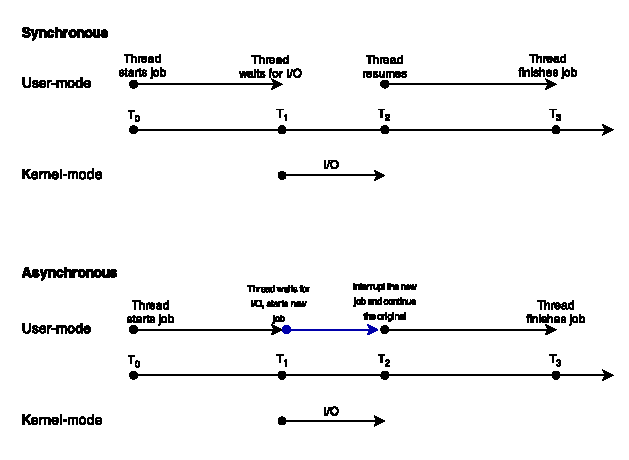
\includegraphics[scale=1.2]{billeder/sync-async.pdf}  
  \caption{Synchronous and asyncronous execution. Based on \cite{ms-syn-asyn}.}
  \label{fig:syncasync}
\end{figure}

This is the case for one or few users, but if there are many users at once they either have to wait in queue for previous I/O operations to finish, or each operation has to be executed in it's own thread, which would potentially result in many active threads, requiring a lot of memory. As pointed out by \citet{amir} it is worth noting that an asynchronous call that results in a synchronous operation causes the application to block, and therefore should be considered during implementation.

To enable the server to scale better, the I/O is implemented asynchronously. When the server receives an input, it is asynchronously sent to a dispatcher which sends it to the correct place; this is described in \Cref{sec:server}. Because of the many parts that have to interact, it is hard to determine if this implementation behaves as expected without testing it, but changing to a synchronous implementation would not be very expensive, as the asynchronous code is very similar to the synchronous code thanks to .NET's \texttt{Async} and \texttt{Await} keywords \cite{ms-asyn}. Making both implementations available at the same time, and letting the user choose which one to use, would also be relatively easy to do, but it adds some extra complexity to the code, as changes in one implementation would require similar changes in the other.
%What are the advantages and disadvantages?

%Which alternative(s) is/are there?

%Why did we make the choice we did?

%How flexible is it?
% - Could it easily be changed? 
% - Could both be implemented and the framework-user decides which one to use?
%
%\section{Synchronous vs. Asynchronous I/O}\fxfatal{This section will be rewritten with proper sources.}
%For the client/server socket communication, a choice between synchronous and asynchronous I/O has to be taken.
%% % blocking % %
%Synchronous I/O can have a better performance than asynchronous, but can cause problems when using a threaded architecture that spawns a new thread for each client. This is particularly true when the server should be scalable in regards to its number of connected clients. There might be 5 and there might be 5000 or even more.
%Tests show that threads are very efficient when it comes to memory and context switching, but only when the threads are kept alive for the entire execution of an application. This is not the case for our application, which will likely have many connections of varying durations during its up-time. \fixme{cite}\\\\
%% % non-blocking % %
%Asynchronous I/O is chosen for this project. It scales well when there are many clients, and the system should scale well with a potentially large number of clients. A notable advantage of asynchronous is that it limits the number of concurrent threads. The server asynchronously accepts a connection request from a client, and then starts an asynchronous worker thread to handle communication with the client. Meanwhile it continues to listen for new client connections.
%

%The ability to scale well does not come for free, however. Non-blocking IO is not always as fast as blocking IO and this can result in decreased performance. 
\section{Model View Controller}
%Describe why an architectural pattern is important

%We chose MVC - describe it

%What do we gain from MVC? What are the tradeoffs?

%Other options? Model-View-Presenter, Observer, Multitier architecture?

%Is it possible to change the architecture?
\section{Design Patterns}
When considering how to design a software solution it can be a good idea to consider using some design patterns. Without those, code easily becomes messy later on in the project. Patterns can help by providing conventions and best practices to use as guidelines. With defined patterns it can be ensured that everyone working on the project has similar understandings of the code. It is worth to note that like everything, patterns can be misused; It is important to choose those that will fit the project, rather than try to force harmful patterns on to it. 

Below is a description of patterns found usable in this project. Patterns are split into two, one with patterns applicable in the client application, another with patterns applicable on the server program.

\subsection{Patterns in the application}
\textbf{Singleton} was an obvious pattern to use in the application for certain elements. Firstly, the application including all activities are singleton. This is enforced by Android. There is no reason why the user should run multiple instances of the game. A certain class called "Client" is however also important to keep singleton. This class is responsible for opening a connection to the server and handle communication. It should not be allowed for a user to send multiple requests to the server at once.

\textbf{Lazy Initialization} have been used to save some resources. Why the application does not perform any major operations, it should always be remembered that it is running on a phone and that it has a battery. As such, most initializations of objects has been pushed back to the point where they are required.

\textbf{Adapter} pattern is used to construct lists, grids and the like in Android. The adapters are used to display items using a given layout to inflate and a set of items. It will then provide a view of each item, effectively providing a user-friendly way of using the data. For this project adapters have been used to create and display clickable lists.

\textbf{Facade} pattern has been used mostly for abstracting server communication with the server. As this is done by creating XML strings with relevant data, this would be tedious to do in every activity that needed server communication. The communication itself was also abstracted. Instead, this functionality has been written in separate classes. An example can be seen in \ref{fig:facadepattern}. This displays what happens when a user tries to login. The username and password is converted to XML and sent to the server, which then responds. All the details of how this happens are however hidden.

\begin{figure}[H]
\centering
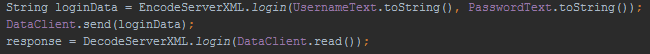
\includegraphics[width=\textwidth]{billeder/facadepattern.png}
\caption{Abstraction of server communication}
\label{fig:facadepattern}
\end{figure} 

\subsection{Patterns on server}
% If you are about to write about thread pool, we are not using a thread pool. We just make a thread for each game.

% for pattern in project:
	%Describe each pattern we use:
	% - What is its purpose?
	% - Pros/cons?
	% - Alternatives?
	% - Flexibility (refactoring, adding new functionality, changing the pattern...)
\section{Server Architecture}
%The purpose of this section is to describe the overall architecture of the server.

% Something like:

%		Client
%		------
%Server:  IO
%       [] [] [] [] []...
%     [Game1] [Game 2] ... [Game n]   [MENU/LOGIN]
%     []  []  []  [] []...
%        [DB]

% Class diagram

% Database schema

\subsection{Database}
The database is designed with flexibility in mind which means it is up the game logic to interpret the data in the database. \figref{fig:ER}\fxwarning{export new ER diagram} shows the entity relation diagram for the database without attributes. The database is structured as follows:

\begin{figure}
  \centering
  % Graphic for TeX using PGF
% \usepackage{tikz}
% The following commands are not supported in PSTricks at present
% We define them conditionally, so when they are implemented,
% this pgf file will use them.
\ifx\du\undefined
  \newlength{\du}
\fi
\setlength{\du}{15\unitlength}
\begin{tikzpicture}
\pgftransformxscale{0.700000}
\pgftransformyscale{-1.000000}
\definecolor{dialinecolor}{rgb}{0.000000, 0.000000, 0.000000}
\pgfsetstrokecolor{dialinecolor}
\definecolor{dialinecolor}{rgb}{1.000000, 1.000000, 1.000000}
\pgfsetfillcolor{dialinecolor}
\definecolor{dialinecolor}{rgb}{1.000000, 1.000000, 1.000000}
\pgfsetfillcolor{dialinecolor}
\fill (-8.000000\du,-6.000000\du)--(-8.000000\du,-4.200000\du)--(-3.905000\du,-4.200000\du)--(-3.905000\du,-6.000000\du)--cycle;
\pgfsetlinewidth{0.100000\du}
\pgfsetdash{}{0pt}
\pgfsetmiterjoin
\definecolor{dialinecolor}{rgb}{0.000000, 0.000000, 0.000000}
\pgfsetstrokecolor{dialinecolor}
\draw (-8.000000\du,-6.000000\du)--(-8.000000\du,-4.200000\du)--(-3.905000\du,-4.200000\du)--(-3.905000\du,-6.000000\du)--cycle;
% setfont left to latex
\definecolor{dialinecolor}{rgb}{0.000000, 0.000000, 0.000000}
\pgfsetstrokecolor{dialinecolor}
\node at (-5.952500\du,-4.900000\du){Account};
\definecolor{dialinecolor}{rgb}{1.000000, 1.000000, 1.000000}
\pgfsetfillcolor{dialinecolor}
\fill (18.600000\du,-7.150000\du)--(18.600000\du,-5.350000\du)--(21.540000\du,-5.350000\du)--(21.540000\du,-7.150000\du)--cycle;
\pgfsetlinewidth{0.100000\du}
\pgfsetdash{}{0pt}
\pgfsetmiterjoin
\definecolor{dialinecolor}{rgb}{0.000000, 0.000000, 0.000000}
\pgfsetstrokecolor{dialinecolor}
\draw (18.600000\du,-7.150000\du)--(18.600000\du,-5.350000\du)--(21.540000\du,-5.350000\du)--(21.540000\du,-7.150000\du)--cycle;
% setfont left to latex
\definecolor{dialinecolor}{rgb}{0.000000, 0.000000, 0.000000}
\pgfsetstrokecolor{dialinecolor}
\node at (20.070000\du,-6.050000\du){Game};
\definecolor{dialinecolor}{rgb}{1.000000, 1.000000, 1.000000}
\pgfsetfillcolor{dialinecolor}
\fill (21.200000\du,1.750000\du)--(21.200000\du,3.550000\du)--(24.140000\du,3.550000\du)--(24.140000\du,1.750000\du)--cycle;
\pgfsetlinewidth{0.100000\du}
\pgfsetdash{}{0pt}
\pgfsetmiterjoin
\definecolor{dialinecolor}{rgb}{0.000000, 0.000000, 0.000000}
\pgfsetstrokecolor{dialinecolor}
\draw (21.200000\du,1.750000\du)--(21.200000\du,3.550000\du)--(24.140000\du,3.550000\du)--(24.140000\du,1.750000\du)--cycle;
% setfont left to latex
\definecolor{dialinecolor}{rgb}{0.000000, 0.000000, 0.000000}
\pgfsetstrokecolor{dialinecolor}
\node at (22.670000\du,2.850000\du){Team};
% setfont left to latex
\definecolor{dialinecolor}{rgb}{0.000000, 0.000000, 0.000000}
\pgfsetstrokecolor{dialinecolor}
\node[anchor=west] at (22.670000\du,2.650000\du){};
\definecolor{dialinecolor}{rgb}{1.000000, 1.000000, 1.000000}
\pgfsetfillcolor{dialinecolor}
\fill (13.000000\du,-2.360500\du)--(15.732500\du,-4.000000\du)--(18.465000\du,-2.360500\du)--(15.732500\du,-0.721000\du)--cycle;
\pgfsetlinewidth{0.100000\du}
\pgfsetdash{}{0pt}
\pgfsetmiterjoin
\definecolor{dialinecolor}{rgb}{0.000000, 0.000000, 0.000000}
\pgfsetstrokecolor{dialinecolor}
\draw (13.000000\du,-2.360500\du)--(15.732500\du,-4.000000\du)--(18.465000\du,-2.360500\du)--(15.732500\du,-0.721000\du)--cycle;
% setfont left to latex
\definecolor{dialinecolor}{rgb}{0.000000, 0.000000, 0.000000}
\pgfsetstrokecolor{dialinecolor}
\node[anchor=east] at (12.700000\du,-2.660500\du){1};
\definecolor{dialinecolor}{rgb}{0.000000, 0.000000, 0.000000}
\pgfsetstrokecolor{dialinecolor}
\node[anchor=west] at (18.765000\du,-2.660500\du){N};
\definecolor{dialinecolor}{rgb}{0.000000, 0.000000, 0.000000}
\pgfsetstrokecolor{dialinecolor}
\node at (15.732500\du,-2.160500\du){Inventory};
\definecolor{dialinecolor}{rgb}{1.000000, 1.000000, 1.000000}
\pgfsetfillcolor{dialinecolor}
\fill (21.100000\du,-3.250000\du)--(21.100000\du,-1.450000\du)--(24.040000\du,-1.450000\du)--(24.040000\du,-3.250000\du)--cycle;
\pgfsetlinewidth{0.100000\du}
\pgfsetdash{}{0pt}
\pgfsetmiterjoin
\definecolor{dialinecolor}{rgb}{0.000000, 0.000000, 0.000000}
\pgfsetstrokecolor{dialinecolor}
\draw (21.100000\du,-3.250000\du)--(21.100000\du,-1.450000\du)--(24.040000\du,-1.450000\du)--(24.040000\du,-3.250000\du)--cycle;
% setfont left to latex
\definecolor{dialinecolor}{rgb}{0.000000, 0.000000, 0.000000}
\pgfsetstrokecolor{dialinecolor}
\node at (22.570000\du,-2.150000\du){Item};
\definecolor{dialinecolor}{rgb}{1.000000, 1.000000, 1.000000}
\pgfsetfillcolor{dialinecolor}
\fill (26.500000\du,-2.325999\du)--(29.040000\du,-3.849999\du)--(31.580000\du,-2.325999\du)--(29.040000\du,-0.801999\du)--cycle;
\pgfsetlinewidth{0.100000\du}
\pgfsetdash{}{0pt}
\pgfsetmiterjoin
\definecolor{dialinecolor}{rgb}{0.000000, 0.000000, 0.000000}
\pgfsetstrokecolor{dialinecolor}
\draw (26.500000\du,-2.325999\du)--(29.040000\du,-3.849999\du)--(31.580000\du,-2.325999\du)--(29.040000\du,-0.801999\du)--cycle;
% setfont left to latex
\definecolor{dialinecolor}{rgb}{0.000000, 0.000000, 0.000000}
\pgfsetstrokecolor{dialinecolor}
\node[anchor=east] at (26.200000\du,-2.625999\du){1};
\definecolor{dialinecolor}{rgb}{0.000000, 0.000000, 0.000000}
\pgfsetstrokecolor{dialinecolor}
\node[anchor=west] at (31.880000\du,-2.625999\du){1};
\definecolor{dialinecolor}{rgb}{0.000000, 0.000000, 0.000000}
\pgfsetstrokecolor{dialinecolor}
\node at (29.040000\du,-2.125999\du){has\_item};
\definecolor{dialinecolor}{rgb}{1.000000, 1.000000, 1.000000}
\pgfsetfillcolor{dialinecolor}
\fill (33.900000\du,-3.250000\du)--(33.900000\du,-1.450000\du)--(38.380000\du,-1.450000\du)--(38.380000\du,-3.250000\du)--cycle;
\pgfsetlinewidth{0.100000\du}
\pgfsetdash{}{0pt}
\pgfsetmiterjoin
\definecolor{dialinecolor}{rgb}{0.000000, 0.000000, 0.000000}
\pgfsetstrokecolor{dialinecolor}
\draw (33.900000\du,-3.250000\du)--(33.900000\du,-1.450000\du)--(38.380000\du,-1.450000\du)--(38.380000\du,-3.250000\du)--cycle;
% setfont left to latex
\definecolor{dialinecolor}{rgb}{0.000000, 0.000000, 0.000000}
\pgfsetstrokecolor{dialinecolor}
\node at (36.140000\du,-2.150000\du){Location};
\definecolor{dialinecolor}{rgb}{1.000000, 1.000000, 1.000000}
\pgfsetfillcolor{dialinecolor}
\fill (27.200004\du,2.627500\du)--(29.162504\du,1.450000\du)--(31.125004\du,2.627500\du)--(29.162504\du,3.805000\du)--cycle;
\pgfsetlinewidth{0.100000\du}
\pgfsetdash{}{0pt}
\pgfsetmiterjoin
\definecolor{dialinecolor}{rgb}{0.000000, 0.000000, 0.000000}
\pgfsetstrokecolor{dialinecolor}
\draw (27.200004\du,2.627500\du)--(29.162504\du,1.450000\du)--(31.125004\du,2.627500\du)--(29.162504\du,3.805000\du)--cycle;
% setfont left to latex
\definecolor{dialinecolor}{rgb}{0.000000, 0.000000, 0.000000}
\pgfsetstrokecolor{dialinecolor}
\node[anchor=east] at (26.900004\du,2.327500\du){1};
\definecolor{dialinecolor}{rgb}{0.000000, 0.000000, 0.000000}
\pgfsetstrokecolor{dialinecolor}
\node[anchor=west] at (31.425004\du,2.327500\du){N};
\definecolor{dialinecolor}{rgb}{0.000000, 0.000000, 0.000000}
\pgfsetstrokecolor{dialinecolor}
\node at (29.162504\du,2.827500\du){holds};
\definecolor{dialinecolor}{rgb}{1.000000, 1.000000, 1.000000}
\pgfsetfillcolor{dialinecolor}
\fill (26.900004\du,-6.268999\du)--(28.285004\du,-7.099999\du)--(29.670004\du,-6.268999\du)--(28.285004\du,-5.437999\du)--cycle;
\pgfsetlinewidth{0.100000\du}
\pgfsetdash{}{0pt}
\pgfsetmiterjoin
\definecolor{dialinecolor}{rgb}{0.000000, 0.000000, 0.000000}
\pgfsetstrokecolor{dialinecolor}
\draw (26.900004\du,-6.268999\du)--(28.285004\du,-7.099999\du)--(29.670004\du,-6.268999\du)--(28.285004\du,-5.437999\du)--cycle;
% setfont left to latex
\definecolor{dialinecolor}{rgb}{0.000000, 0.000000, 0.000000}
\pgfsetstrokecolor{dialinecolor}
\node[anchor=east] at (26.600004\du,-6.568999\du){1};
\definecolor{dialinecolor}{rgb}{0.000000, 0.000000, 0.000000}
\pgfsetstrokecolor{dialinecolor}
\node[anchor=west] at (29.970004\du,-6.568999\du){N};
\definecolor{dialinecolor}{rgb}{0.000000, 0.000000, 0.000000}
\pgfsetstrokecolor{dialinecolor}
\node at (28.285004\du,-6.068999\du){in};
\definecolor{dialinecolor}{rgb}{1.000000, 1.000000, 1.000000}
\pgfsetfillcolor{dialinecolor}
\fill (-1.000000\du,-8.822500\du)--(0.962500\du,-10.000000\du)--(2.925000\du,-8.822500\du)--(0.962500\du,-7.645000\du)--cycle;
\pgfsetlinewidth{0.100000\du}
\pgfsetdash{}{0pt}
\pgfsetmiterjoin
\definecolor{dialinecolor}{rgb}{0.000000, 0.000000, 0.000000}
\pgfsetstrokecolor{dialinecolor}
\draw (-1.000000\du,-8.822500\du)--(0.962500\du,-10.000000\du)--(2.925000\du,-8.822500\du)--(0.962500\du,-7.645000\du)--cycle;
% setfont left to latex
\definecolor{dialinecolor}{rgb}{0.000000, 0.000000, 0.000000}
\pgfsetstrokecolor{dialinecolor}
\node[anchor=east] at (-1.300000\du,-9.122500\du){1};
\definecolor{dialinecolor}{rgb}{0.000000, 0.000000, 0.000000}
\pgfsetstrokecolor{dialinecolor}
\node[anchor=west] at (3.225000\du,-9.122500\du){N};
\definecolor{dialinecolor}{rgb}{0.000000, 0.000000, 0.000000}
\pgfsetstrokecolor{dialinecolor}
\node at (0.962500\du,-8.622500\du){hosts};
\definecolor{dialinecolor}{rgb}{1.000000, 1.000000, 1.000000}
\pgfsetfillcolor{dialinecolor}
\fill (6.900000\du,-3.250001\du)--(6.900000\du,-1.450001\du)--(10.610000\du,-1.450001\du)--(10.610000\du,-3.250001\du)--cycle;
\pgfsetlinewidth{0.100000\du}
\pgfsetdash{}{0pt}
\pgfsetmiterjoin
\definecolor{dialinecolor}{rgb}{0.000000, 0.000000, 0.000000}
\pgfsetstrokecolor{dialinecolor}
\draw (6.900000\du,-3.250001\du)--(6.900000\du,-1.450001\du)--(10.610000\du,-1.450001\du)--(10.610000\du,-3.250001\du)--cycle;
% setfont left to latex
\definecolor{dialinecolor}{rgb}{0.000000, 0.000000, 0.000000}
\pgfsetstrokecolor{dialinecolor}
\node at (8.755000\du,-2.150001\du){Player};
\definecolor{dialinecolor}{rgb}{1.000000, 1.000000, 1.000000}
\pgfsetfillcolor{dialinecolor}
\fill (-1.000000\du,-5.088000\du)--(0.770000\du,-6.150000\du)--(2.540000\du,-5.088000\du)--(0.770000\du,-4.026000\du)--cycle;
\pgfsetlinewidth{0.100000\du}
\pgfsetdash{}{0pt}
\pgfsetmiterjoin
\definecolor{dialinecolor}{rgb}{0.000000, 0.000000, 0.000000}
\pgfsetstrokecolor{dialinecolor}
\draw (-1.000000\du,-5.088000\du)--(0.770000\du,-6.150000\du)--(2.540000\du,-5.088000\du)--(0.770000\du,-4.026000\du)--cycle;
% setfont left to latex
\definecolor{dialinecolor}{rgb}{0.000000, 0.000000, 0.000000}
\pgfsetstrokecolor{dialinecolor}
\node[anchor=east] at (-1.300000\du,-5.388000\du){1};
\definecolor{dialinecolor}{rgb}{0.000000, 0.000000, 0.000000}
\pgfsetstrokecolor{dialinecolor}
\node[anchor=west] at (2.840000\du,-5.388000\du){N};
\definecolor{dialinecolor}{rgb}{0.000000, 0.000000, 0.000000}
\pgfsetstrokecolor{dialinecolor}
\node at (0.770000\du,-4.888000\du){owns};
\definecolor{dialinecolor}{rgb}{1.000000, 1.000000, 1.000000}
\pgfsetfillcolor{dialinecolor}
\fill (10.350000\du,-6.269000\du)--(11.735000\du,-7.100000\du)--(13.120000\du,-6.269000\du)--(11.735000\du,-5.438000\du)--cycle;
\pgfsetlinewidth{0.100000\du}
\pgfsetdash{}{0pt}
\pgfsetmiterjoin
\definecolor{dialinecolor}{rgb}{0.000000, 0.000000, 0.000000}
\pgfsetstrokecolor{dialinecolor}
\draw (10.350000\du,-6.269000\du)--(11.735000\du,-7.100000\du)--(13.120000\du,-6.269000\du)--(11.735000\du,-5.438000\du)--cycle;
% setfont left to latex
\definecolor{dialinecolor}{rgb}{0.000000, 0.000000, 0.000000}
\pgfsetstrokecolor{dialinecolor}
\node[anchor=east] at (10.050000\du,-6.569000\du){N};
\definecolor{dialinecolor}{rgb}{0.000000, 0.000000, 0.000000}
\pgfsetstrokecolor{dialinecolor}
\node[anchor=west] at (13.420000\du,-6.569000\du){1};
\definecolor{dialinecolor}{rgb}{0.000000, 0.000000, 0.000000}
\pgfsetstrokecolor{dialinecolor}
\node at (11.735000\du,-6.069000\du){in};
\pgfsetlinewidth{0.100000\du}
\pgfsetdash{}{0pt}
\pgfsetdash{}{0pt}
\pgfsetbuttcap
{
\definecolor{dialinecolor}{rgb}{0.000000, 0.000000, 0.000000}
\pgfsetfillcolor{dialinecolor}
% was here!!!
\definecolor{dialinecolor}{rgb}{0.000000, 0.000000, 0.000000}
\pgfsetstrokecolor{dialinecolor}
\draw (13.120000\du,-6.269000\du)--(18.600000\du,-6.250000\du);
}
\definecolor{dialinecolor}{rgb}{1.000000, 1.000000, 1.000000}
\pgfsetfillcolor{dialinecolor}
\fill (10.000000\du,2.639500\du)--(12.732500\du,1.000000\du)--(15.465000\du,2.639500\du)--(12.732500\du,4.279000\du)--cycle;
\pgfsetlinewidth{0.100000\du}
\pgfsetdash{}{0pt}
\pgfsetmiterjoin
\definecolor{dialinecolor}{rgb}{0.000000, 0.000000, 0.000000}
\pgfsetstrokecolor{dialinecolor}
\draw (10.000000\du,2.639500\du)--(12.732500\du,1.000000\du)--(15.465000\du,2.639500\du)--(12.732500\du,4.279000\du)--cycle;
% setfont left to latex
\definecolor{dialinecolor}{rgb}{0.000000, 0.000000, 0.000000}
\pgfsetstrokecolor{dialinecolor}
\node[anchor=east] at (9.700000\du,2.339500\du){N};
\definecolor{dialinecolor}{rgb}{0.000000, 0.000000, 0.000000}
\pgfsetstrokecolor{dialinecolor}
\node[anchor=west] at (15.765000\du,2.339500\du){1};
\definecolor{dialinecolor}{rgb}{0.000000, 0.000000, 0.000000}
\pgfsetstrokecolor{dialinecolor}
\node at (12.732500\du,2.839500\du){is\_member};
\definecolor{dialinecolor}{rgb}{1.000000, 1.000000, 1.000000}
\pgfsetfillcolor{dialinecolor}
\fill (-7.700000\du,-0.949999\du)--(-7.700000\du,0.850001\du)--(-1.295000\du,0.850001\du)--(-1.295000\du,-0.949999\du)--cycle;
\pgfsetlinewidth{0.100000\du}
\pgfsetdash{}{0pt}
\pgfsetmiterjoin
\definecolor{dialinecolor}{rgb}{0.000000, 0.000000, 0.000000}
\pgfsetstrokecolor{dialinecolor}
\draw (-7.700000\du,-0.949999\du)--(-7.700000\du,0.850001\du)--(-1.295000\du,0.850001\du)--(-1.295000\du,-0.949999\du)--cycle;
\definecolor{dialinecolor}{rgb}{0.000000, 0.000000, 0.000000}
\pgfsetstrokecolor{dialinecolor}
\draw (-7.450000\du,-0.699999\du)--(-7.450000\du,0.600001\du)--(-1.545000\du,0.600001\du)--(-1.545000\du,-0.699999\du)--cycle;
% setfont left to latex
\definecolor{dialinecolor}{rgb}{0.000000, 0.000000, 0.000000}
\pgfsetstrokecolor{dialinecolor}
\node at (-4.497500\du,0.150001\du){Status Effect};
\definecolor{dialinecolor}{rgb}{1.000000, 1.000000, 1.000000}
\pgfsetfillcolor{dialinecolor}
\fill (1.000000\du,-0.053500\du)--(2.577500\du,-1.000000\du)--(4.155000\du,-0.053500\du)--(2.577500\du,0.893000\du)--cycle;
\pgfsetlinewidth{0.100000\du}
\pgfsetdash{}{0pt}
\pgfsetmiterjoin
\definecolor{dialinecolor}{rgb}{0.000000, 0.000000, 0.000000}
\pgfsetstrokecolor{dialinecolor}
\draw (1.000000\du,-0.053500\du)--(2.577500\du,-1.000000\du)--(4.155000\du,-0.053500\du)--(2.577500\du,0.893000\du)--cycle;
\definecolor{dialinecolor}{rgb}{0.000000, 0.000000, 0.000000}
\pgfsetstrokecolor{dialinecolor}
\draw (1.400000\du,-0.053500\du)--(2.577500\du,-0.760000\du)--(3.755000\du,-0.053500\du)--(2.577500\du,0.653000\du)--cycle;
% setfont left to latex
\definecolor{dialinecolor}{rgb}{0.000000, 0.000000, 0.000000}
\pgfsetstrokecolor{dialinecolor}
\node[anchor=east] at (0.700000\du,-0.353500\du){N};
\definecolor{dialinecolor}{rgb}{0.000000, 0.000000, 0.000000}
\pgfsetstrokecolor{dialinecolor}
\node[anchor=west] at (4.455000\du,-0.353500\du){1};
\definecolor{dialinecolor}{rgb}{0.000000, 0.000000, 0.000000}
\pgfsetstrokecolor{dialinecolor}
\node at (2.577500\du,0.146500\du){has};
\pgfsetlinewidth{0.100000\du}
\pgfsetdash{}{0pt}
\pgfsetdash{}{0pt}
\pgfsetmiterjoin
\pgfsetbuttcap
{
\definecolor{dialinecolor}{rgb}{0.000000, 0.000000, 0.000000}
\pgfsetfillcolor{dialinecolor}
% was here!!!
{\pgfsetcornersarced{\pgfpoint{0.000000\du}{0.000000\du}}\definecolor{dialinecolor}{rgb}{0.000000, 0.000000, 0.000000}
\pgfsetstrokecolor{dialinecolor}
\draw (20.070000\du,-7.150000\du)--(20.070000\du,-8.749106\du)--(2.925000\du,-8.749106\du)--(2.925000\du,-8.822500\du);
}}
\pgfsetlinewidth{0.100000\du}
\pgfsetdash{}{0pt}
\pgfsetdash{}{0pt}
\pgfsetmiterjoin
\pgfsetbuttcap
{
\definecolor{dialinecolor}{rgb}{0.000000, 0.000000, 0.000000}
\pgfsetfillcolor{dialinecolor}
% was here!!!
{\pgfsetcornersarced{\pgfpoint{0.000000\du}{0.000000\du}}\definecolor{dialinecolor}{rgb}{0.000000, 0.000000, 0.000000}
\pgfsetstrokecolor{dialinecolor}
\draw (-1.000000\du,-8.822500\du)--(-1.000000\du,-8.799106\du)--(-5.952500\du,-8.799106\du)--(-5.952500\du,-6.000000\du);
}}
\pgfsetlinewidth{0.100000\du}
\pgfsetdash{}{0pt}
\pgfsetdash{}{0pt}
\pgfsetmiterjoin
\pgfsetbuttcap
{
\definecolor{dialinecolor}{rgb}{0.000000, 0.000000, 0.000000}
\pgfsetfillcolor{dialinecolor}
% was here!!!
{\pgfsetcornersarced{\pgfpoint{0.000000\du}{0.000000\du}}\definecolor{dialinecolor}{rgb}{0.000000, 0.000000, 0.000000}
\pgfsetstrokecolor{dialinecolor}
\draw (-1.000000\du,-5.088000\du)--(-2.452500\du,-5.088000\du)--(-2.452500\du,-5.100000\du)--(-3.905000\du,-5.100000\du);
}}
\pgfsetlinewidth{0.100000\du}
\pgfsetdash{}{0pt}
\pgfsetdash{}{0pt}
\pgfsetmiterjoin
\pgfsetbuttcap
{
\definecolor{dialinecolor}{rgb}{0.000000, 0.000000, 0.000000}
\pgfsetfillcolor{dialinecolor}
% was here!!!
{\pgfsetcornersarced{\pgfpoint{0.000000\du}{0.000000\du}}\definecolor{dialinecolor}{rgb}{0.000000, 0.000000, 0.000000}
\pgfsetstrokecolor{dialinecolor}
\draw (2.540000\du,-5.088000\du)--(4.720000\du,-5.088000\du)--(4.720000\du,-2.350001\du)--(6.900000\du,-2.350001\du);
}}
\pgfsetlinewidth{0.100000\du}
\pgfsetdash{}{0pt}
\pgfsetdash{}{0pt}
\pgfsetmiterjoin
\pgfsetbuttcap
{
\definecolor{dialinecolor}{rgb}{0.000000, 0.000000, 0.000000}
\pgfsetfillcolor{dialinecolor}
% was here!!!
{\pgfsetcornersarced{\pgfpoint{0.000000\du}{0.000000\du}}\definecolor{dialinecolor}{rgb}{0.000000, 0.000000, 0.000000}
\pgfsetstrokecolor{dialinecolor}
\draw (10.350000\du,-6.269000\du)--(10.350000\du,-6.199108\du)--(8.755000\du,-6.199108\du)--(8.755000\du,-3.299591\du);
}}
\pgfsetlinewidth{0.100000\du}
\pgfsetdash{}{0pt}
\pgfsetdash{}{0pt}
\pgfsetmiterjoin
\pgfsetbuttcap
{
\definecolor{dialinecolor}{rgb}{0.000000, 0.000000, 0.000000}
\pgfsetfillcolor{dialinecolor}
% was here!!!
{\pgfsetcornersarced{\pgfpoint{0.000000\du}{0.000000\du}}\definecolor{dialinecolor}{rgb}{0.000000, 0.000000, 0.000000}
\pgfsetstrokecolor{dialinecolor}
\draw (6.849535\du,-2.350001\du)--(5.527070\du,-2.350001\du)--(5.527070\du,-0.053500\du)--(4.204606\du,-0.053500\du);
}}
\pgfsetlinewidth{0.100000\du}
\pgfsetdash{}{0pt}
\pgfsetdash{}{0pt}
\pgfsetmiterjoin
\pgfsetbuttcap
{
\definecolor{dialinecolor}{rgb}{0.000000, 0.000000, 0.000000}
\pgfsetfillcolor{dialinecolor}
% was here!!!
{\pgfsetcornersarced{\pgfpoint{0.000000\du}{0.000000\du}}\definecolor{dialinecolor}{rgb}{0.000000, 0.000000, 0.000000}
\pgfsetstrokecolor{dialinecolor}
\draw (12.952405\du,-2.360500\du)--(11.806435\du,-2.360500\du)--(11.806435\du,-2.350001\du)--(10.660465\du,-2.350001\du);
}}
\pgfsetlinewidth{0.100000\du}
\pgfsetdash{}{0pt}
\pgfsetdash{}{0pt}
\pgfsetmiterjoin
\pgfsetbuttcap
{
\definecolor{dialinecolor}{rgb}{0.000000, 0.000000, 0.000000}
\pgfsetfillcolor{dialinecolor}
% was here!!!
{\pgfsetcornersarced{\pgfpoint{0.000000\du}{0.000000\du}}\definecolor{dialinecolor}{rgb}{0.000000, 0.000000, 0.000000}
\pgfsetstrokecolor{dialinecolor}
\draw (21.049629\du,-2.350000\du)--(19.781112\du,-2.350000\du)--(19.781112\du,-2.360500\du)--(18.512595\du,-2.360500\du);
}}
\pgfsetlinewidth{0.100000\du}
\pgfsetdash{}{0pt}
\pgfsetdash{}{0pt}
\pgfsetmiterjoin
\pgfsetbuttcap
{
\definecolor{dialinecolor}{rgb}{0.000000, 0.000000, 0.000000}
\pgfsetfillcolor{dialinecolor}
% was here!!!
{\pgfsetcornersarced{\pgfpoint{0.000000\du}{0.000000\du}}\definecolor{dialinecolor}{rgb}{0.000000, 0.000000, 0.000000}
\pgfsetstrokecolor{dialinecolor}
\draw (24.090371\du,-2.350000\du)--(25.271496\du,-2.350000\du)--(25.271496\du,-2.325999\du)--(26.452622\du,-2.325999\du);
}}
\pgfsetlinewidth{0.100000\du}
\pgfsetdash{}{0pt}
\pgfsetdash{}{0pt}
\pgfsetmiterjoin
\pgfsetbuttcap
{
\definecolor{dialinecolor}{rgb}{0.000000, 0.000000, 0.000000}
\pgfsetfillcolor{dialinecolor}
% was here!!!
{\pgfsetcornersarced{\pgfpoint{0.000000\du}{0.000000\du}}\definecolor{dialinecolor}{rgb}{0.000000, 0.000000, 0.000000}
\pgfsetstrokecolor{dialinecolor}
\draw (21.590371\du,-6.250000\du)--(24.220066\du,-6.250000\du)--(24.220066\du,-6.268999\du)--(26.849760\du,-6.268999\du);
}}
\pgfsetlinewidth{0.100000\du}
\pgfsetdash{}{0pt}
\pgfsetdash{}{0pt}
\pgfsetmiterjoin
\pgfsetbuttcap
{
\definecolor{dialinecolor}{rgb}{0.000000, 0.000000, 0.000000}
\pgfsetfillcolor{dialinecolor}
% was here!!!
{\pgfsetcornersarced{\pgfpoint{0.000000\du}{0.000000\du}}\definecolor{dialinecolor}{rgb}{0.000000, 0.000000, 0.000000}
\pgfsetstrokecolor{dialinecolor}
\draw (36.140000\du,-3.250000\du)--(36.140000\du,-6.249108\du)--(29.670004\du,-6.249108\du)--(29.670004\du,-6.268999\du);
}}
\pgfsetlinewidth{0.100000\du}
\pgfsetdash{}{0pt}
\pgfsetdash{}{0pt}
\pgfsetmiterjoin
\pgfsetbuttcap
{
\definecolor{dialinecolor}{rgb}{0.000000, 0.000000, 0.000000}
\pgfsetfillcolor{dialinecolor}
% was here!!!
{\pgfsetcornersarced{\pgfpoint{0.000000\du}{0.000000\du}}\definecolor{dialinecolor}{rgb}{0.000000, 0.000000, 0.000000}
\pgfsetstrokecolor{dialinecolor}
\draw (31.627378\du,-2.325999\du)--(32.738549\du,-2.325999\du)--(32.738549\du,-2.350000\du)--(33.849721\du,-2.350000\du);
}}
\pgfsetlinewidth{0.100000\du}
\pgfsetdash{}{0pt}
\pgfsetdash{}{0pt}
\pgfsetmiterjoin
\pgfsetbuttcap
{
\definecolor{dialinecolor}{rgb}{0.000000, 0.000000, 0.000000}
\pgfsetfillcolor{dialinecolor}
% was here!!!
{\pgfsetcornersarced{\pgfpoint{0.000000\du}{0.000000\du}}\definecolor{dialinecolor}{rgb}{0.000000, 0.000000, 0.000000}
\pgfsetstrokecolor{dialinecolor}
\draw (21.149629\du,2.650000\du)--(18.331112\du,2.650000\du)--(18.331112\du,2.639500\du)--(15.512595\du,2.639500\du);
}}
\pgfsetlinewidth{0.100000\du}
\pgfsetdash{}{0pt}
\pgfsetdash{}{0pt}
\pgfsetmiterjoin
\pgfsetbuttcap
{
\definecolor{dialinecolor}{rgb}{0.000000, 0.000000, 0.000000}
\pgfsetfillcolor{dialinecolor}
% was here!!!
{\pgfsetcornersarced{\pgfpoint{0.000000\du}{0.000000\du}}\definecolor{dialinecolor}{rgb}{0.000000, 0.000000, 0.000000}
\pgfsetstrokecolor{dialinecolor}
\draw (24.190371\du,2.650000\du)--(25.672778\du,2.650000\du)--(25.672778\du,2.627500\du)--(27.155184\du,2.627500\du);
}}
\pgfsetlinewidth{0.100000\du}
\pgfsetdash{}{0pt}
\pgfsetdash{}{0pt}
\pgfsetmiterjoin
\pgfsetbuttcap
{
\definecolor{dialinecolor}{rgb}{0.000000, 0.000000, 0.000000}
\pgfsetfillcolor{dialinecolor}
% was here!!!
{\pgfsetcornersarced{\pgfpoint{0.000000\du}{0.000000\du}}\definecolor{dialinecolor}{rgb}{0.000000, 0.000000, 0.000000}
\pgfsetstrokecolor{dialinecolor}
\draw (-1.244603\du,-0.049999\du)--(-0.147104\du,-0.049999\du)--(-0.147104\du,-0.053500\du)--(0.950394\du,-0.053500\du);
}}
\pgfsetlinewidth{0.100000\du}
\pgfsetdash{}{0pt}
\pgfsetdash{}{0pt}
\pgfsetmiterjoin
\pgfsetbuttcap
{
\definecolor{dialinecolor}{rgb}{0.000000, 0.000000, 0.000000}
\pgfsetfillcolor{dialinecolor}
% was here!!!
{\pgfsetcornersarced{\pgfpoint{0.000000\du}{0.000000\du}}\definecolor{dialinecolor}{rgb}{0.000000, 0.000000, 0.000000}
\pgfsetstrokecolor{dialinecolor}
\draw (8.755000\du,-1.399820\du)--(8.755000\du,2.650885\du)--(10.000000\du,2.650885\du)--(10.000000\du,2.639500\du);
}}
\pgfsetlinewidth{0.100000\du}
\pgfsetdash{}{0pt}
\pgfsetdash{}{0pt}
\pgfsetmiterjoin
\pgfsetbuttcap
{
\definecolor{dialinecolor}{rgb}{0.000000, 0.000000, 0.000000}
\pgfsetfillcolor{dialinecolor}
% was here!!!
{\pgfsetcornersarced{\pgfpoint{0.000000\du}{0.000000\du}}\definecolor{dialinecolor}{rgb}{0.000000, 0.000000, 0.000000}
\pgfsetstrokecolor{dialinecolor}
\draw (36.140000\du,-1.399820\du)--(36.140000\du,2.650885\du)--(31.125004\du,2.650885\du)--(31.125004\du,2.627500\du);
}}
\end{tikzpicture}
  
  \caption{ER Diagram.}
  \label{fig:ER}
\end{figure}




\paragraph{Account}
The Account entity represent the users in the system. An account can host games represented by the host relation and take part in games represented as owning a player in a particular game.

\paragraph{Player}
This entity represent a user playing in a game. A player can hold items, have status effects and be a member of a team represented by Inventory, has(Status Effect) and Team(is\_member) respectively. The player entity also contains score and location etc. for a particular player in a game.

\paragraph{Game}
This entity represent games either \textit{starting up}, \textit{in progress} and \textit{ended}.

\paragraph{Status Effect}
Effects on a player is represented by this entity. An effect could be \textit{disabled until time} on a particular player. Status Effects have an effect type which the game logic is responsible for defining.

\paragraph{Team}
Players can be members of teams in a game, though a player is not required to be on a team to allow free for all game modes.


\paragraph{Item}
Items represent any object in the inventory of players or on a location in the game world. Items can be anything from objects players can ``pick up'' to a capturable area in the game world. The attributes and behavior of items are defined by game logic.

\paragraph{Location}
A location is an item in the game world can belong to a team or no teams.

\subsection{Game thread-pool}
The game thread-pool is a collection of active game thread-instances, uniquely identified by a game-Id.

The game thread-pool is used as a handle to the game threads, and allows dynamic call to the desired game through method-parametrization. 

\subsection{Game thread}
\paragraph{Starting a game}
A game thread will be initialised and started when a user requests to host a game. A game will be assigned a game-id by the server, user-specified settings for hosting the game will be initialised and the game will be created in the database. 

When the server initialises each setting, it calls a method within the game thread-class. These methods calls the database-controller to change the state of the game in the database. These settings are:
\begin{itemize}
\item Game-privacy (Public or private game)
\item Number of teams
\item Game start-time
\item Game end-time
\item Game-boundary NorthWest GPS-coordinate
\item Game-boundary SouthEast GPS-coordinate
\end{itemize}

\paragraph{Updating a game}
Updates to a game can be split into two groups. One group is specific changes to a game, like inviting a new player or firing a gun. Another group is updating a players position when moving around in the game.

Updating a players position is trivial. The game thread receives a game-id, player-id and a new position. It calls the database-controller to store the new position in the database.

When performing an action like firing a gun, the server will have to fetch the gunman's position and the victim's position. It will then calculate if the range of the fired weapon allows the victim to be hit. If the shot is successful it will return that to the player, if the shot is unsuccessful it will return that the victim is out of range. 

All updates to change the state of a game will be in the game thread-class. This class will need to contain methods for all the in-game functionality. 

\paragraph{Closing a game}
When a game ends, the call will come from the timer thread. This will ask the game thread to clean up what is has stored in the database, and return a status message. The timer thread will then continue to close the game thread. 




\section{Interfaces}
%INTRO:
%Server and client both consist of several small parts that all need to communicate.
%Examples: user->client, client->server, game->db...

We have decided that all information between the server and the client are shared in the form of XML. We have chosen to do so because of the diversity XML provides, and its interoperability with a wide variety of software. This fits well within the theme of creating a very customizable framework for creating games. Furthermore we feel that XML is somewhat of a standard for sharing - and many people already know how to make use of it.

\subsection{Client and Server correspondence}

The idea behind the XML output is to create tags for each different kind of data. We have different kinds of data to sent depending on which activity we take on the client side. An example of this could be the login activity on the client side, this requires sending some username and a password for confirmation on the server side.

We create individual methods for each different scenario rather than creating a generic XML converter because we want to enforce the right data structures and types. The example below is the said convert to XML login method. 

\begin{lstlisting}
    public static String login(String username, String password) {

        String tag = "Login";
        String entryA = "Username";
        String entryB = "Password";

        String xml = "";

        xml += "<" + tag + ">";
        xml += "<" + entryA + ">" + username + "</" + entryA + ">";
        xml += "<" + entryB + ">" + password + "</" + entryB + ">";
        xml += "</" + tag + ">";

        return xml;
    }
\end{lstlisting}

It simply converts the input of the variables username and password into XML on the form (except it being on a single string). The information is structured around what the server needs for authentication - so what the client sends is of course built around what the server requires.

\begin{lstlsting}
<Login>
   <Username> USERNAME </Username>
   <Password> PASSWORD </Password>
</Login>
\end{lstlisting}

A basic principle of TCP is that the client always require a response from server before it can move on. For the same reasons mentioned above and for the sake of consistency the client expects XML on roughly the same form. For this example we require an ID for the specific user to load his specific settings/information. We also require a boolean in the case that it wasn't a valid login, this is then handled on the client side. The following code is what a client expects to receive.

\begin{lstlisting}
<Login>
   <Id> IDENTIFICATION </Id>
   <Valid> BOOL </Valid>
</Login>
\end{lstlisting}

XML provides a really easy way to dispatch or deserialize the input - making it an optimal solution for small constant interactions like the ones we need. There are many different alternatives to XML, but we feel that it is a simple interaction without extraordinarily complicated needs - which makes the simplicity of XML a great trait for us.

%PROJECT IMPACT:
%Several sub-groups are developing the different parts, so...
%How does this need for communication impact development?

%We chose to do *like this* - why did we choose that, and was it a good choice, or would something else have been better?

%SOLUTION
%How is this communication done? (How are the interfaces made, and how was it decided?)

%Why is it done like this? Is it efficient? Easy? Scalable? Maintainable? Something else?

%Are there any alternatives? Why not one of them?
\section{Game Rules}
%Why did we make game rules?

%What are pros and cons of making them? (aka how do they help us, how do they limit us?)

%Write the game rules.

%Discuss how easily a different set of rules could be implemented
\section{Seperation of Framework and Game}
%It should be possbile to build a new game on the same framework.
The framework and the game is split into two completely seperate components. This enables creation of a new game on the same framework. 
%Why is the framework and game seperated?
The reason for this choice, is that the framework can be reused for different games. Because of this future developers who would like to make a game can reuse the framework and do not have to touch any framework code, only the game code itself. 
%Why is it a good idea, and what are the tradeoffs?
Developing the framework and game as two completely independent components has a number of good side effects. First of all, it makes it easier to avoid writing code which is intertwined (between the framework and the game). 
%What would happen if it is not split up?
If this was not avoided, it would be very hard to create an independent framework, since part og the game which was developed on top of the framework would be tied into the framework and vice versa. Therefore, a clear code-wise distinction between framework and server produces cleaner, more independent overall program structure. 
%Discuss the constraints of the framework (e.g. database schema, efficiency).
Because the framework and game are separated components, the framework has some limitations. The framework essentially enables development of many kinds of networked multiplayer games. Therefore, the database's tables for example have to be quite ``fixed'', since the developers of the games for the framework should not need to change the database and framework code. A database change will likely warrant some code in the framework to be rewritten. If the developers have to start rewriting code in the framework to develop their game, the point of the framework is lost. 

%\chapter{Prototypes}
\label{chap:proto}

\section{Downloading based on signal strength}
\label{sec:sigstr}

downloading map of deadzone when the signal strength is dwindling.\newpage
\section{Dangerzone based on analysis}
\label{sec:dgrzone}

The thought behind this idea is simple and easy to implement given we have the information needed to do the analysis. The idea is to design a heat map based on some sort of information - in this example we will be using location of radio towers and  the location of forests. Whenever two signals overlap the ``heat'' would rise in that section as illustrated in figure \ref{fig:tempdgr_1}. In our example forests obstruct signal, therefore creating less signal on the opposing side of the forest, this is illustrated in \ref{fig:tempdgr_2}. With these implications we can build the entire map based on information gathered before the application is launched. 

\begin{figure} [h!]
        \centering
        \begin{subfigure}[b]{0.45\textwidth}
                \frame{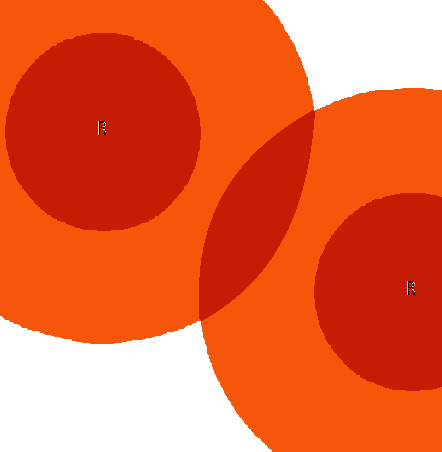
\includegraphics[width=\textwidth]{billeder/tempdgrR}}
                \caption{2 Radiotower signals}
                \label{fig:tempdgr_1}
        \end{subfigure}
        \begin{subfigure}[b]{0.45\textwidth}
                \frame{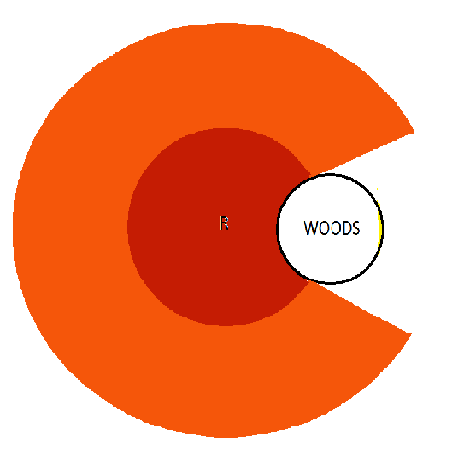
\includegraphics[width=\textwidth]{billeder/tempdgrF}}
                \caption{Signal being obstructed by a forest}
                \label{fig:tempdgr_2}
        \end{subfigure}
        \caption{Illustrations of the idea}\label{fig:temdgr}
\end{figure}


A map designed on different possible aspects (e.g. placement of towers, infrastructure) and not on data collected.


\begin{table} [h]
   \begin{center}
   \begin{minipage}{\textwidth}
      \centering
      \begin{tabularx} {\textwidth} { X | X  }
         \hline
		 & \\
         Advantages & Disadvantages \\
		& \\\hline
		& \\
         \tabitem No data besides the map needs to be saved & \tabitem It assumes there's no unexpected interference\\
         \tabitem The map is built before application launch & \tabitem Requires a lot of information beforehand \\
         \tabitem this is an advantage & \tabitem Requires updates to the map every time new information is out \\
		& \\\hline
      \end{tabularx}
      \caption{this is a dummy}
      \label{tab:dgrzone_adv}
   \end{minipage}
   \end{center}
\end{table}
\newpage
\section{Coverage Maps Based on Crowd Sourced Data}
\label{sec:covmap}

The idea is based on the same premises' as the map based on analysis from section \ref{sec:dgrzone} except it is based on connectivity information gathered from different users. The idea is to have many different devices constantly sending information like coordinates and signal strength. This would create a map which would be based on actual data sent from the devices, and could be updated often based on new datasets. This is a more of an hands on approach to creating a coverage map, as signal strength might vary at unexpected events.

In addition to holding the coordinates up against the created map, as the dangerzone map, this solution needs to send some data which can be saved on the database. It is necessary to send coordinates and signal strength, as they are needed to create the map. Dependant on what information you find important, you can save additional data in the database such as provider or device type.


\begin{table} [h]
   \begin{center}
   \begin{minipage}{\textwidth}
      \centering
      \begin{tabularx} {\textwidth} { X | X  }
         \hline
		 & \\
         Advantages & Disadvantages \\
		& \\\hline
		& \\
         \tabitem highly interchangeable map & \tabitem More data needs to be sent from client side \\
         \tabitem Requires no data prior to implementation & \tabitem Requires a lot of data before the map is usable \\
	 \tabitem It is possible to add additional data to the database & \\
		& \\\hline
      \end{tabularx}
      \caption{this is a dummy}
      \label{tab:dgrzone_adv}
   \end{minipage}
   \end{center}
\end{table}
\newpage
\section{Crowdsourced analysis}
\label{sec:crwdsourc}

Based on nearby devices connection - download map if getting close to zones where a lot of devices don't have connection.

\begin{table} [h]
   \begin{center}
   \begin{minipage}{\textwidth}
      \centering
      \begin{tabularx} {\textwidth} { X | X  }
         \hline
		 & \\
         Advantages & Disadvantages \\
		& \\\hline
		& \\
         \tabitem this is an advantage & \tabitem this an disadvantage \\
         \tabitem this is an advantage & \tabitem this an disadvantage \\
		& \\\hline
      \end{tabularx}
      \caption{this is a dummy}
      \label{tab:dgrzone_adv}
   \end{minipage}
   \end{center}
\end{table}
\newpage
%\chapter{Architechture}
\label{chap:arch}


%%THEORY
%\section{Client and Server connection}

The Transmission Control Protocol (TCP) is a part of the Internet protocol suite. Together with the Internet Protocol (IP), TCP is so widely used that the entire Internet protocol suite, containing many protocols, is often just called TCP/IP.

In the following, the parts of TCP that are particularly important for this project are described. This chapter is based on \cite{wiki-tcp}. \fxfatal{Find better source.}
%Author: Dan, Christoffer
\section{Data Transfer}
%Reliable transfer, error detection
Because we are working with transfer of data to a device with an uncertain connection, it is relevant to consider how TCP handles transferring data. An important aspect of this is to ensure reliable transmission, i.e. to make sure all the data is transferred correctly. To ensure this, each byte of data gets a sequence number, allowing the destination host to reconstruct the data in case of for example packet loss. Additionally, when a packet is received, the receiver sends back an acknowledgement, and if such an acknowledgement is not received the packet will be sent again. To ensure correctness of the packet content, each packet has a checksum included which the packet's content can be compared to upon arrival at its destination.\\

This possibility of error checking comes in handy in our project. When a map is transmitted to a client, it ensures that the map data is not corrupted. This is very desirable since corrupted map data could make the map unusable in the best case, and show wrong map data in the worst case.

\subsection{Flow Control}
It is possible for the server to sent more data than the receiver can process, and to accommodate this a flow control protocol is used. When data is sent, the receiver answers back with a \textit{window size}, telling the sender how much more data it is able to process. If the window size reaches 0, a persist timer will be set to account for the possibility that the updated window size was simply lost. When the timer runs out the server will send a small packet, probing the receiver for an updated window size.

%Should we mention anything about the header overhead?

% Kilde: http://en.wikipedia.org/wiki/Transmission_Control_Protocol#Data_transfer
\subsection{TCP/IP versus UDP}
We would like to consider two aspects of TCP/IP versus UDP. The first aspect is which protocol is cheapest in space usage when transferring from one unit to another. The second aspect is which protocol offers the best suited services for our application.

These questions are related to the problem we try to solve. We want to try to download data on an endangered connection or download within a limited time-span before the device goes offline. Therefore we investigate TCP/IP versus UDP further.

When transferring data from one unit to another, the size of data to send varies depending on the program. However, the header has a minimum or fixed size it always uses, without considering the size of the data the user wants to send. In TCP/IP, the size of the header is 21 octets\cite{tcpdesc}. In UDP, the size of the header is 8 octets\cite{udpdesc}. In comparison, UDP uses 38\% of what TCP/IP uses for each exchange.

The services provided by TCP/IP are reliability through error checking and delivery validation whereas UDP emphasizes low-overhead operation and reduced latency\cite{wiki-tcp}. Both protocols provide valid services to be used when solving our problem. TCP/IP will ensure we have correct, consistent and working data. UDP could be used for transferring GPS-coordinates because they will be transferred extensively when the application is running. Losing an UDP transaction will not break the application. If a few data is lost or inconsistent, new data will be sent in the very near future.
\subsection{Error Detection}
The TCP protocol makes error detection possible. Each packet is assigned a sequence number which enables receivers to ignore duplicate packets and sequence packets which have been reordered, in the right sequence. \fixme{fra wiki: Acknowledgments allow senders to determine when to retransmit lost packets.????????}. To ensure correctness of the packet content, each packet has a checksum included which the packet's content can be compared to upon arrival at its destination.\\

This possibility of error checking comes in handy in our project. When a map is transmitted to a client, it ensures that the map data is not corrupted. This is very desirable since corrupted map data could make the map unusable in the best case, and show wrong map data in the worst case.

%
%%\section{Predicting Signal Loss}
To predict when a device might suffer a signal loss and become disconnected from the internet, two different scenarios must be considered. The scenarios are as follows\\

\begin{itemize}
\item The device is moving into the country side
\item The device is in the city\fxwarning{should this be removed? is the scenario not needed anymore?}
\end{itemize}

In order to predict when the signal may be at risk of being lost in the first scenario, it makes sense to look at measurements from the antenna of the device. A number of measurements, five for example, can then be stored on the device. These values should be error corrected (e.g. using standard deviation) to make sure sudden fluctuations will not trigger an alarm, telling the device that it has lost its signal. Since coverage is usually worse outside of big cities compared to in the cities, the signal will be lost gradually and not suddenly. Therefore it makes sense to measure a number of antenna measurements, and decide whether they are falling at a rate which would indicate being in the country side.\\

In table xxx 
%
%%IMPLEMENTATION
%\chapter{Implementation}
\label{chap:implementation}

%
%%CONCLUSION
%\chapter{Conclusion}
\label{chap:conc}

Here we will describe the result of the entire project, whether it upholds the study regulation. We will also analyse the test results and argue whether they answer the problem statement. We will evaluate the entire project and its functionality as a full program.

\chapter{Conclusion}
\label{chap:conc}

Here we will describe the result of the entire project, whether it upholds the study regulation. We will also analyse the test results and argue whether they answer the problem statement. We will evaluate the entire project and its functionality as a full program.

\chapter{Conclusion}
\label{chap:conc}

Here we will describe the result of the entire project, whether it upholds the study regulation. We will also analyse the test results and argue whether they answer the problem statement. We will evaluate the entire project and its functionality as a full program.

\input{indhold/konklusion/konklusion}
\input{indhold/konklusion/evaluation}
\input{indhold/konklusion/improvements}

%http://thesistips.wordpress.com/2012/03/25/how-to-write-your-introduction-abstract-and-summary/

% It introduces the problem and motivation for the study.
% - Tell the reader what the topic of the report is.
% - Explain why this topic is important or relevant.

% It provides a brief summary of previous engineering and/or scientific work on the topic.
% - Here you present an overview what is known about the problem.  You would typically cite earlier studies conducted on the same topic and/or at this same site, and in doing so, you should reveal the yawning void in the knowledge that your brilliant research will fill.

% It outlines the purpose and specific objectives of the project.

% It provides a ‘road map’ for the rest of the report.
% - This is so that the reader knows what’s coming and sees the logic of your organization.
% - Describe (in approximately one sentence each) the contents of each of the report/thesis chapters.
\section{Evaluation}

\input{indhold/konklusion/evaluation/flexibility}
\section{Improvements}

\input{indhold/konklusion/improvements/server}
\input{indhold/konklusion/improvements/magic}
\input{indhold/konklusion/improvements/magic}

%http://thesistips.wordpress.com/2012/03/25/how-to-write-your-introduction-abstract-and-summary/

% It introduces the problem and motivation for the study.
% - Tell the reader what the topic of the report is.
% - Explain why this topic is important or relevant.

% It provides a brief summary of previous engineering and/or scientific work on the topic.
% - Here you present an overview what is known about the problem.  You would typically cite earlier studies conducted on the same topic and/or at this same site, and in doing so, you should reveal the yawning void in the knowledge that your brilliant research will fill.

% It outlines the purpose and specific objectives of the project.

% It provides a ‘road map’ for the rest of the report.
% - This is so that the reader knows what’s coming and sees the logic of your organization.
% - Describe (in approximately one sentence each) the contents of each of the report/thesis chapters.
\section{Evaluation}

\subsection{Flexibility of Framework}\label{subsec:game-scenarios}
Since we decided create a server with functionality completely independent of the game implemented on top \fxnote{reference til separate frameworks fra server shit}, a lot of different games can be implemented. 

Something simple that could be implemented fast could be a multiplyer pac-man game. Each game would feature one pac-man and several different ghosts. The objective of the game is for the pac-man to collect all the pellets (which could easily be implemented the same way point objectives), and the fruit that makes pac-man chase the ghost would be crates. The server would get fed coordinates and possibly have a live feed of the map on the client side.
Along those lines a multiplayer game like assassins creed could be emulated. A game happening in the Renaissance (with related weapons like crossbows and swords), where each player is a target of another player - and the winner would be guy to first kill his target.

The item system in the database is extremely flexible - they could be weapons as in our example but fit for a certain era or time period. It is completely up to the developer to determine how the weapons are implemented. One could imagine having a theme like the wild west, where everyone only have six-shooters or a close combat game where people only have melee weapons. 

Furthermore the relation between games and teams are 1-N, and this results in us being able to have co-op or free for all games. A king of the hill game seems like a suitable implementation of this, trying to hold shrines while everyone is out to kill you. This means that it would be possible to implement several other popular game-modes like last man standing or deathmatch where you respawn after being killed.

It is also possible to refrain completely from fighting games. An example could be a gather game similar to Googles Ingress, where you get points for having control of certain areas of the map.

There is a lot of different games that easily could be implemented on top of our framework.



\section{Improvements}

\section{Server Architecture}
%The purpose of this section is to describe the overall architecture of the server.

% Something like:

%		Client
%		------
%Server:  IO
%       [] [] [] [] []...
%     [Game1] [Game 2] ... [Game n]   [MENU/LOGIN]
%     []  []  []  [] []...
%        [DB]

% Class diagram

% Database schema

\subsection{Database}
The database is designed with flexibility in mind which means it is up the game logic to interpret the data in the database. \figref{fig:ER}\fxwarning{export new ER diagram} shows the entity relation diagram for the database without attributes. The database is structured as follows:

\begin{figure}
  \centering
  \input{billeder/Server.tex}  
  \caption{ER Diagram.}
  \label{fig:ER}
\end{figure}




\paragraph{Account}
The Account entity represent the users in the system. An account can host games represented by the host relation and take part in games represented as owning a player in a particular game.

\paragraph{Player}
This entity represent a user playing in a game. A player can hold items, have status effects and be a member of a team represented by Inventory, has(Status Effect) and Team(is\_member) respectively. The player entity also contains score and location etc. for a particular player in a game.

\paragraph{Game}
This entity represent games either \textit{starting up}, \textit{in progress} and \textit{ended}.

\paragraph{Status Effect}
Effects on a player is represented by this entity. An effect could be \textit{disabled until time} on a particular player. Status Effects have an effect type which the game logic is responsible for defining.

\paragraph{Team}
Players can be members of teams in a game, though a player is not required to be on a team to allow free for all game modes.


\paragraph{Item}
Items represent any object in the inventory of players or on a location in the game world. Items can be anything from objects players can ``pick up'' to a capturable area in the game world. The attributes and behavior of items are defined by game logic.

\paragraph{Location}
A location is an item in the game world can belong to a team or no teams.

\input{indhold/design/gamethread}




\subsection{Sigende title her}

%
% ex. database gateway improvements
% 
\subsection{Sigende title her}

%
% ex. database gateway improvements
% 

%http://thesistips.wordpress.com/2012/03/25/how-to-write-your-introduction-abstract-and-summary/

% It introduces the problem and motivation for the study.
% - Tell the reader what the topic of the report is.
% - Explain why this topic is important or relevant.

% It provides a brief summary of previous engineering and/or scientific work on the topic.
% - Here you present an overview what is known about the problem.  You would typically cite earlier studies conducted on the same topic and/or at this same site, and in doing so, you should reveal the yawning void in the knowledge that your brilliant research will fill.

% It outlines the purpose and specific objectives of the project.

% It provides a ‘road map’ for the rest of the report.
% - This is so that the reader knows what’s coming and sees the logic of your organization.
% - Describe (in approximately one sentence each) the contents of each of the report/thesis chapters.


\bibliographystyle{chicago}
\bibliography{litteratur/litteratur}

% Appendix
\appendix

\label{LastPage}
\end{document}